\section{\name Prototype Implementation}
\label{sec:prototype}


\begin{figure}[t]
	\begin{center}
		\begin{subfigure}{0.4\textwidth}
		\centering
			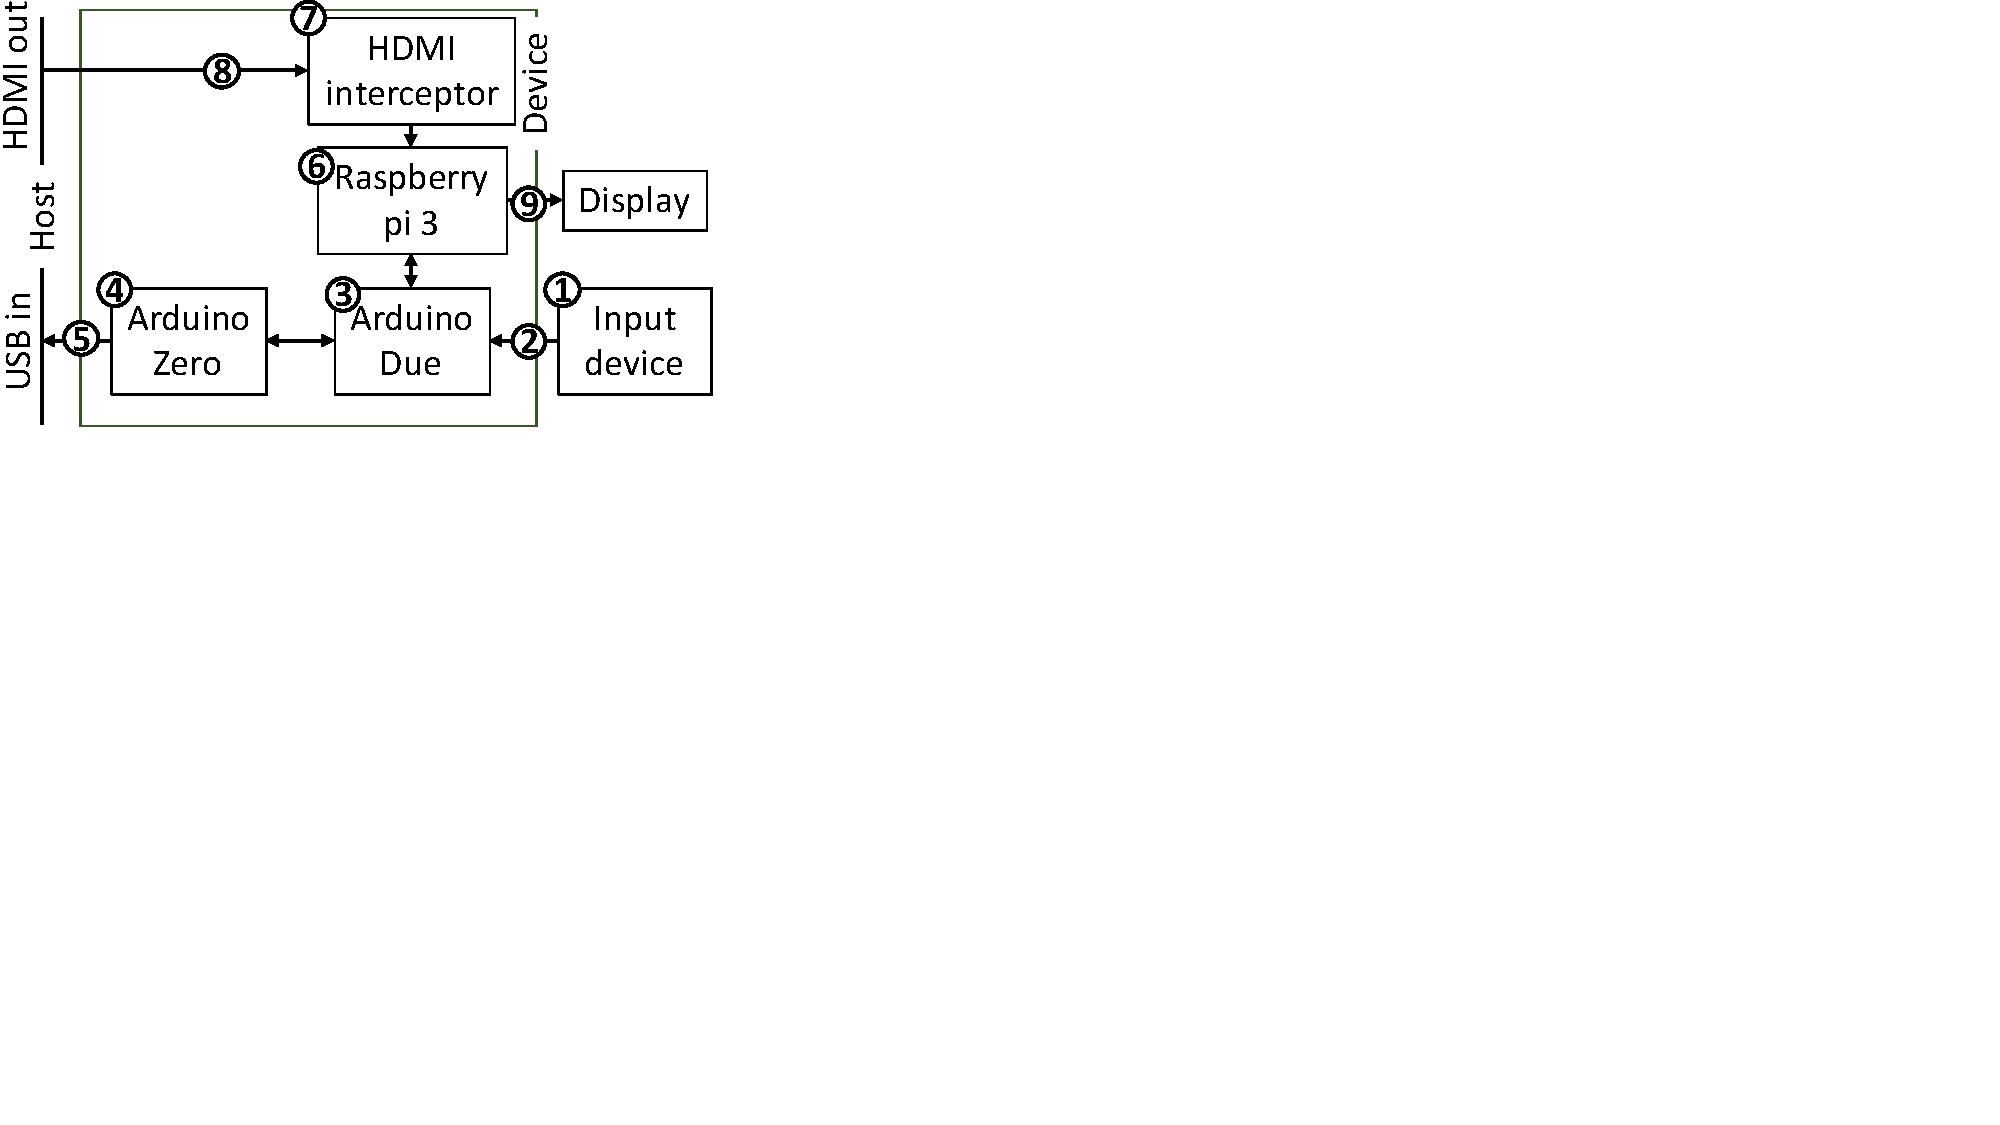
\includegraphics[trim={0 12cm 21.7cm 0}, clip, scale=0.5]{setUpBlock.pdf}
			\caption{The figure shows the basic components and connections between them in our \name prototype.}
			\label{fig:prototypeArch}	
		\end{subfigure}
	\end{center}
	
	%\vspace{1em} 
	
	\begin{center}
		\begin{subfigure}{0.4\textwidth}
		\centering
		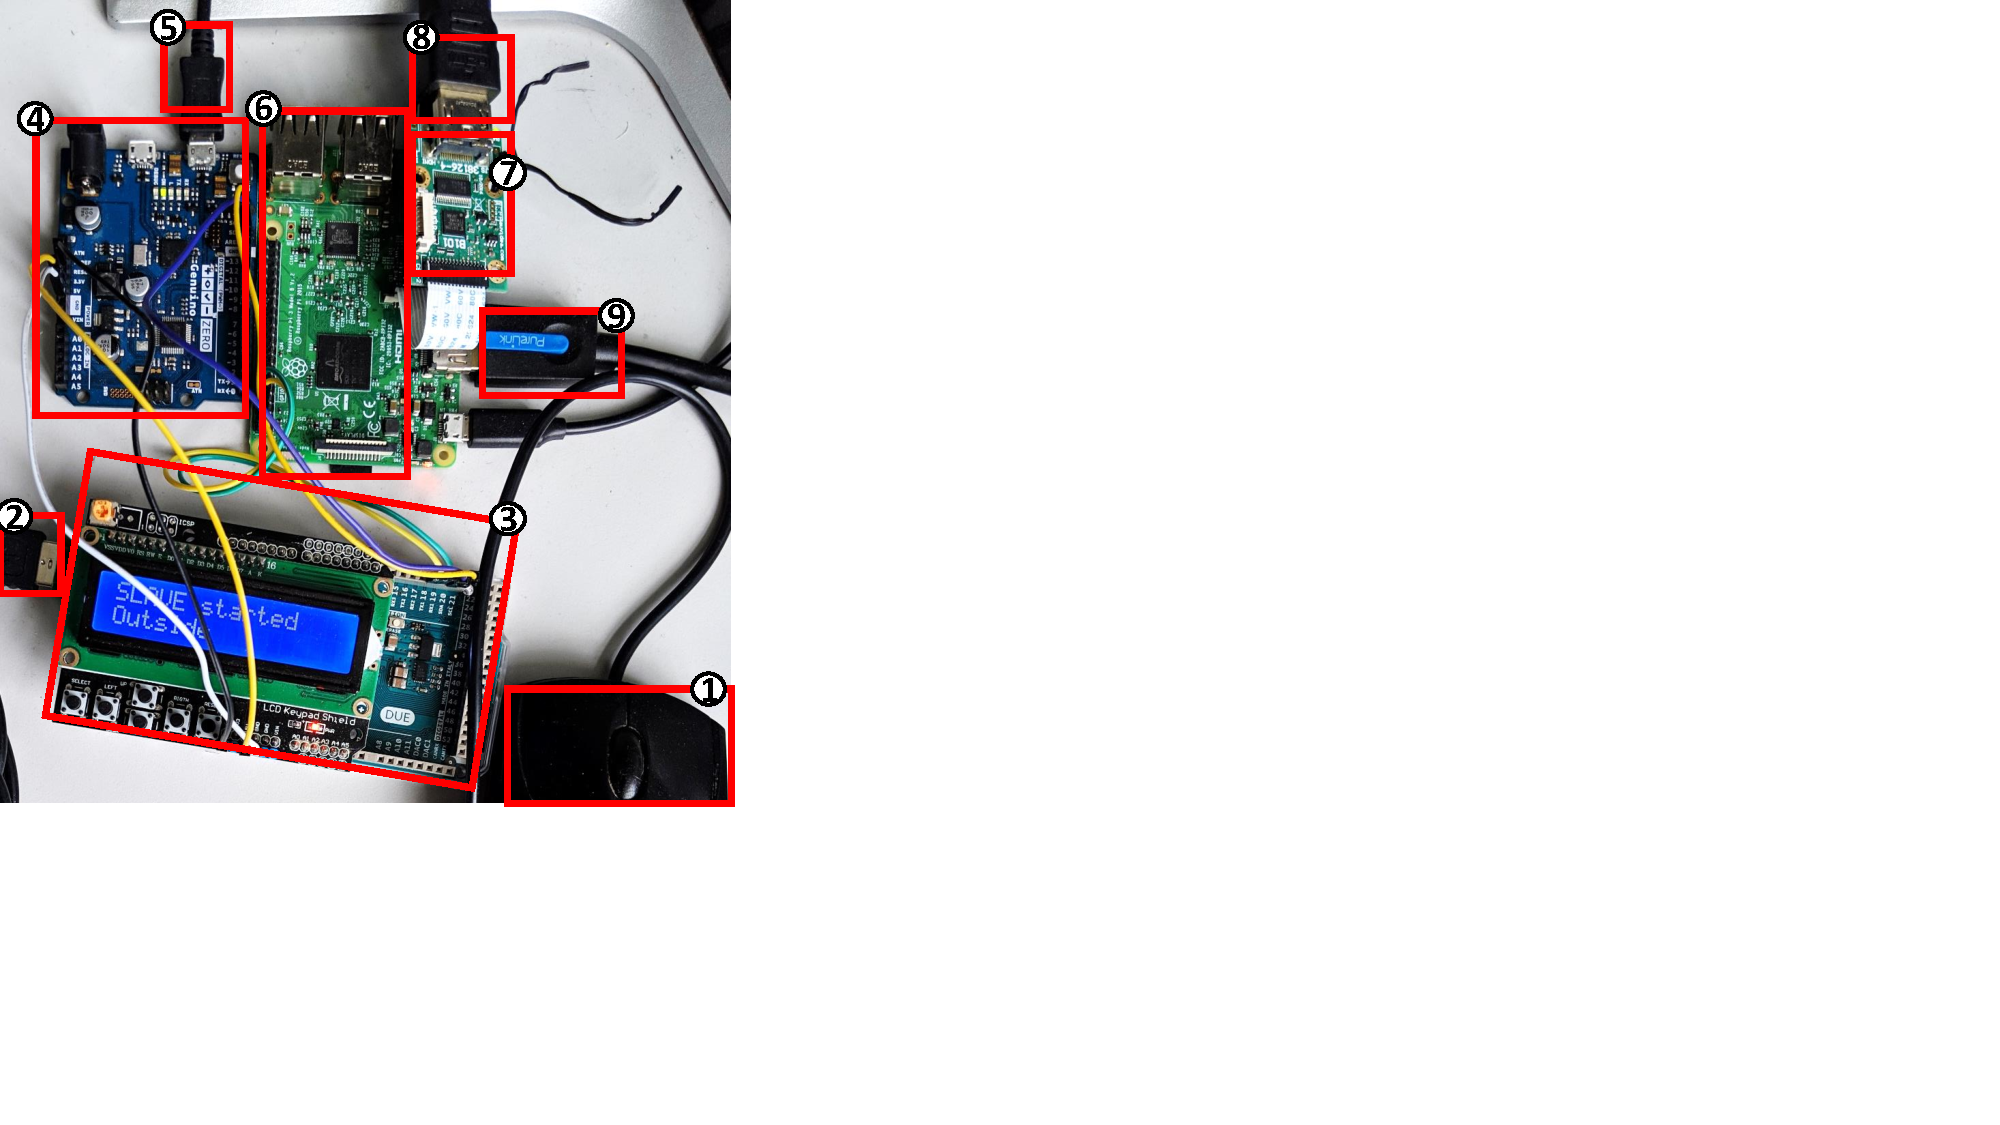
\includegraphics[trim={0 5cm 21.5cm 0}, clip, scale=0.55]{setUp_1.pdf}
		\caption{The figure shows \name prototype that employs Arduino Due and Zero microcontroller board and a Raspberry Pi 3 SBC. The highlighted numbers correspond to the labels in Figure~\ref{fig:prototypeArch}.}
		\label{fig:prototype}
	\end{subfigure}
	\end{center}
	\vspace{-1em}
	\caption{\textbf{\name prototype}. Figure~\ref{fig:prototypeArch} and~\ref{fig:prototype} shows the component diagram and a photo of the actual \name prototype respectively.} 
\end{figure}


\iffalse
\begin{figure}[t]
\centering
%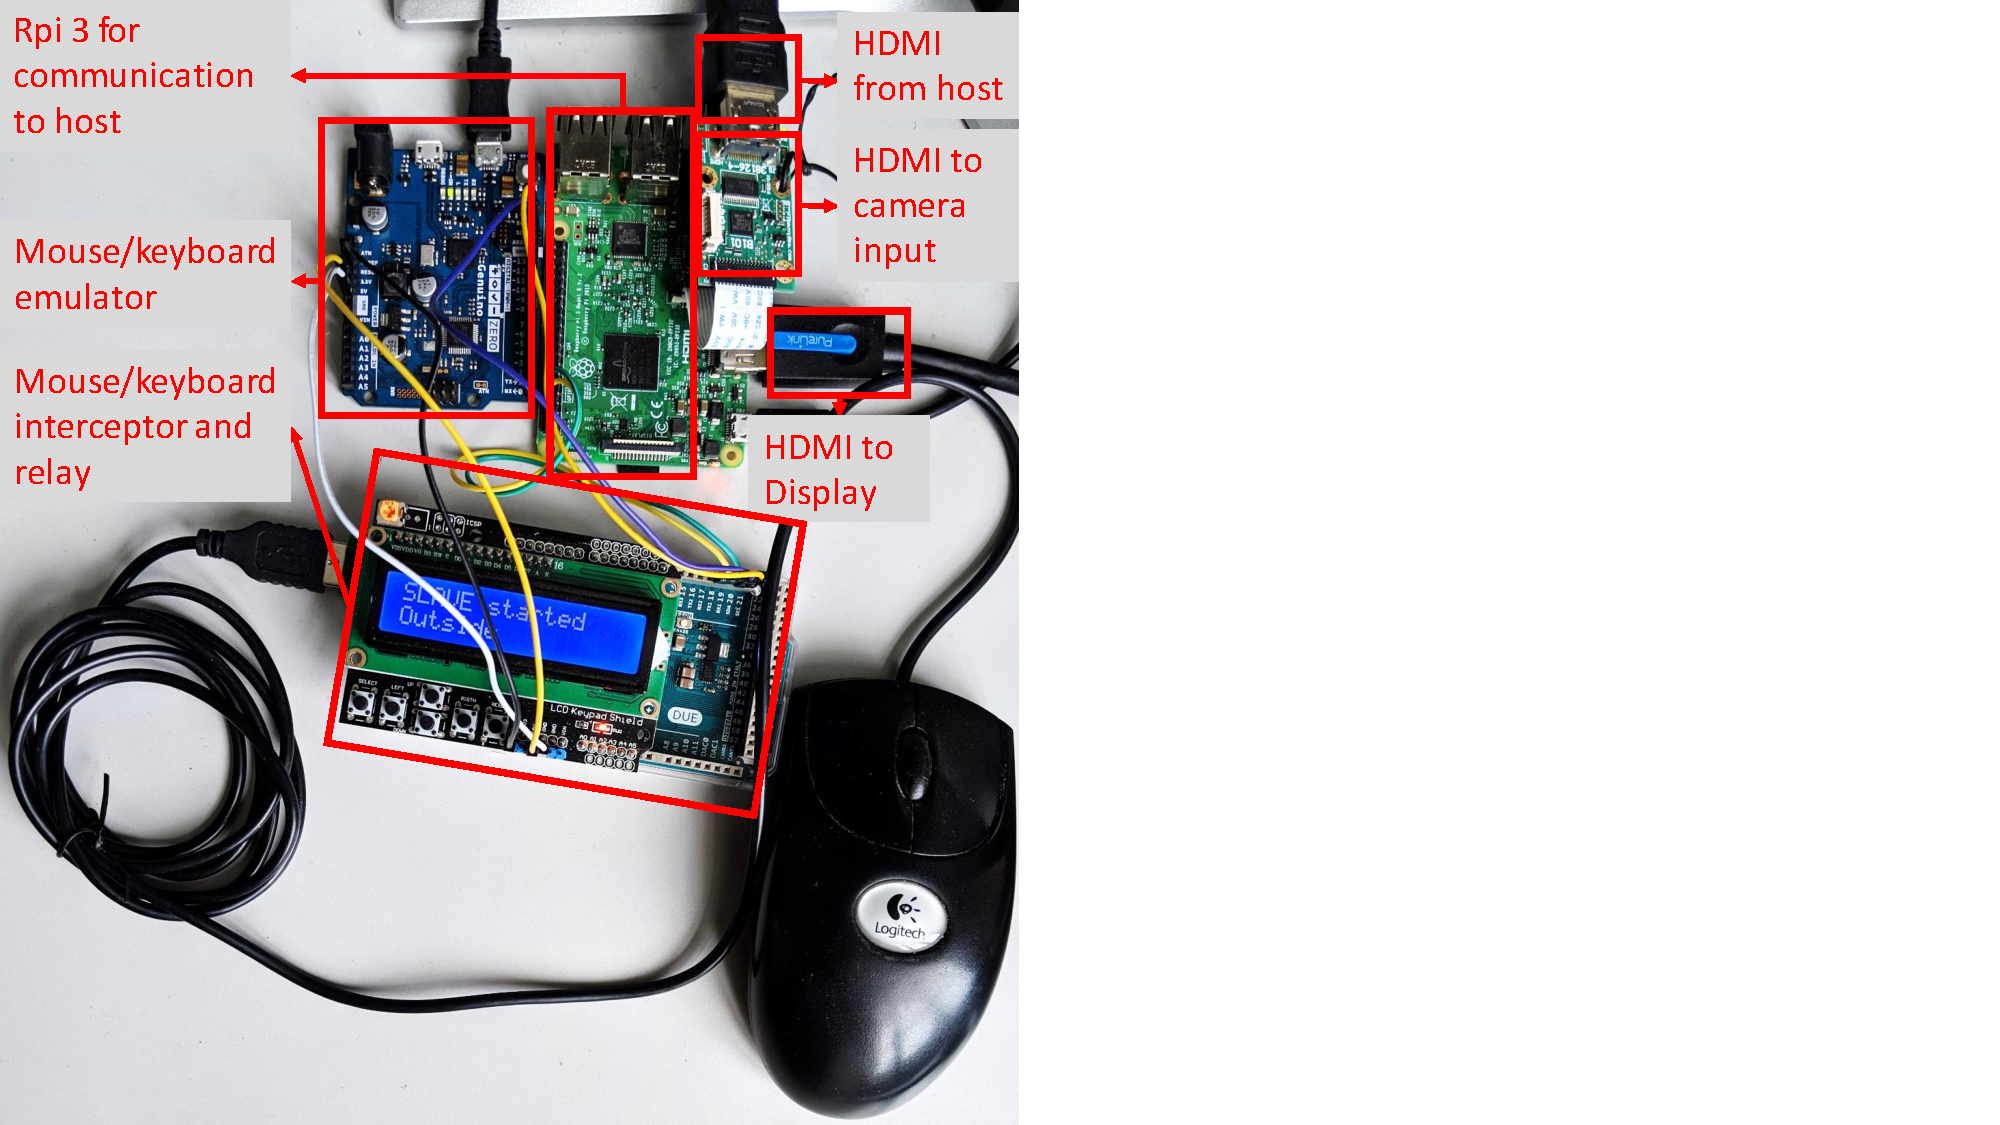
\includegraphics[trim={0 0 15cm 0}, clip, width=\linewidth]{setUp.pdf}
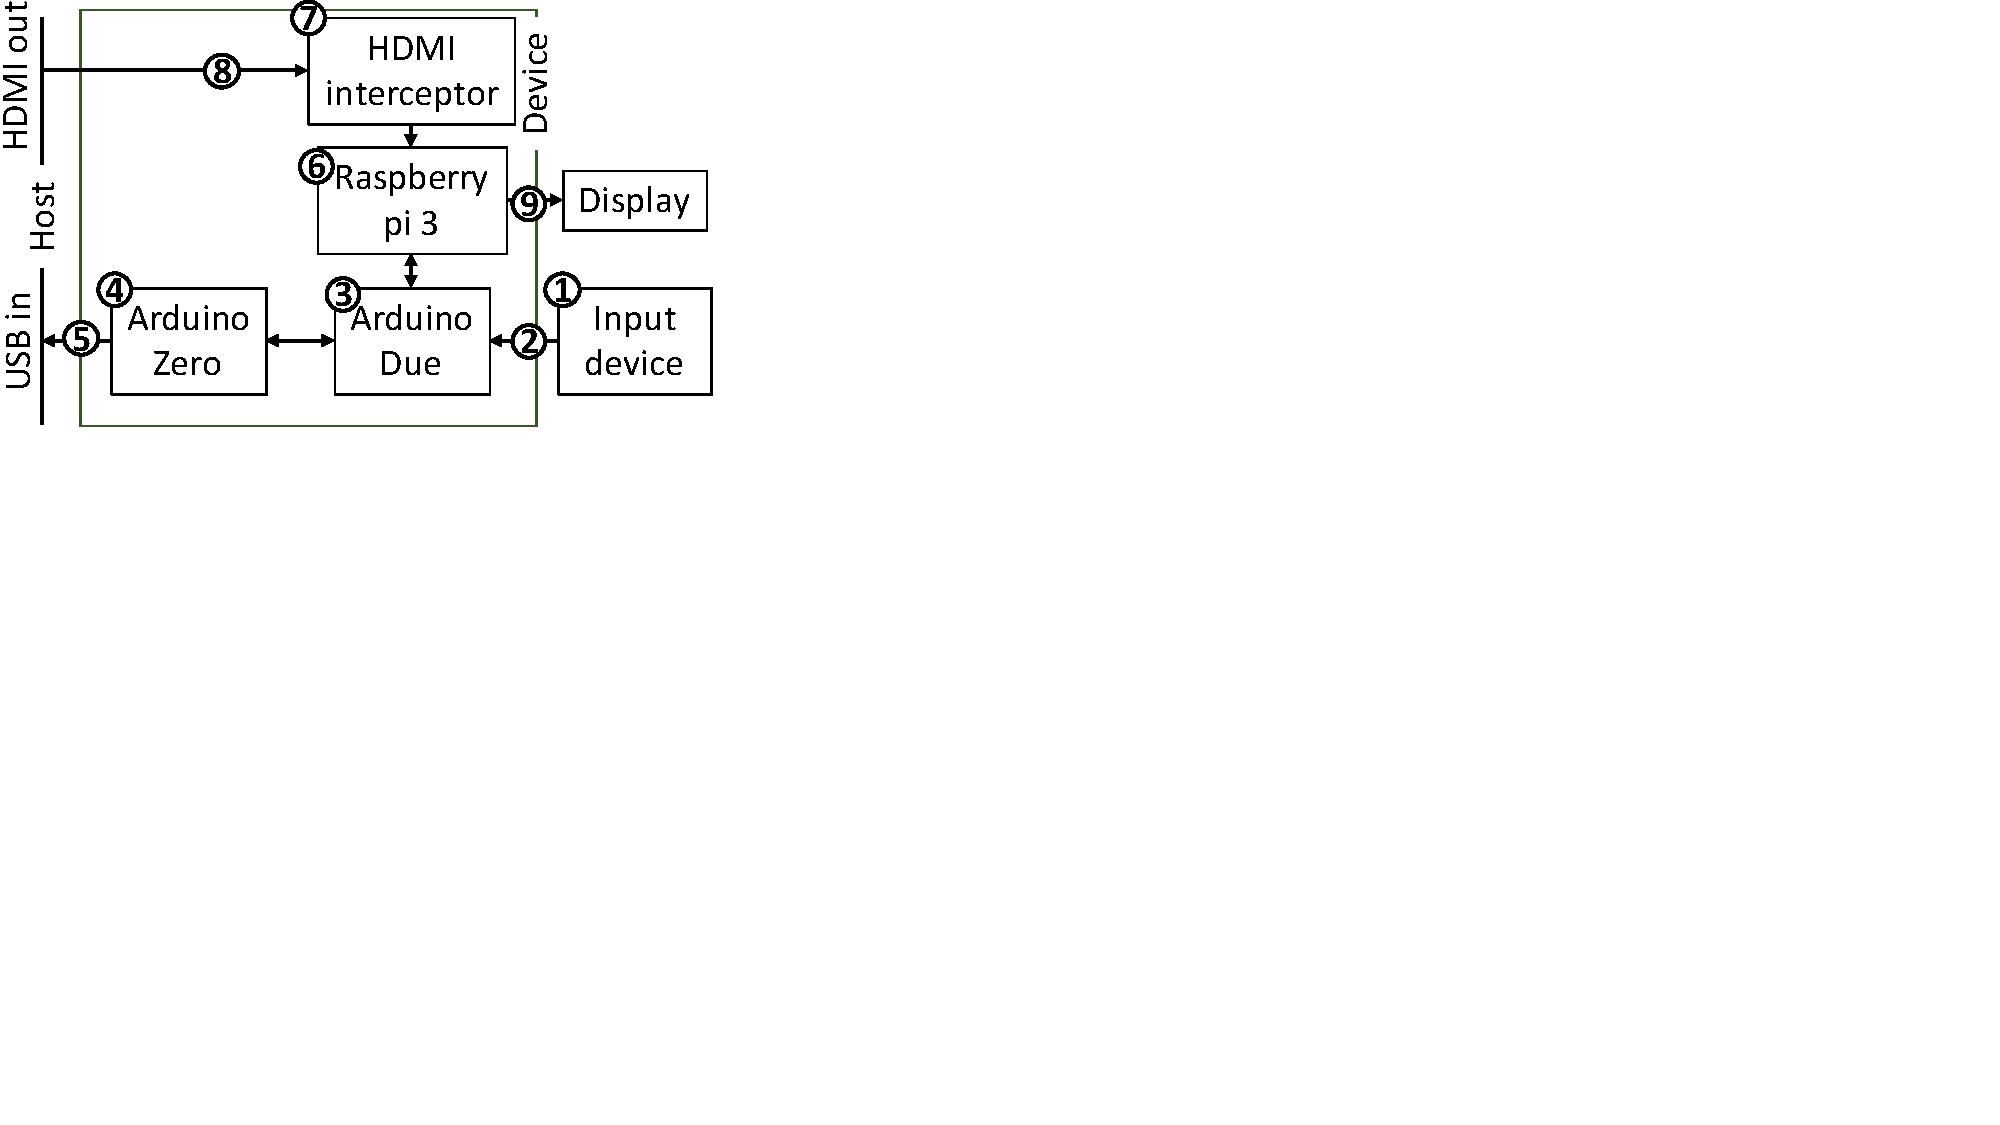
\includegraphics[trim={0 12cm 21.7cm 0}, clip, width=0.65\linewidth]{setUpBlock.pdf}
\caption{\textbf{\name prototype architecture}. }
\label{fig:prototypeArch}
\centering
\end{figure}


\begin{figure}[t]
\centering
%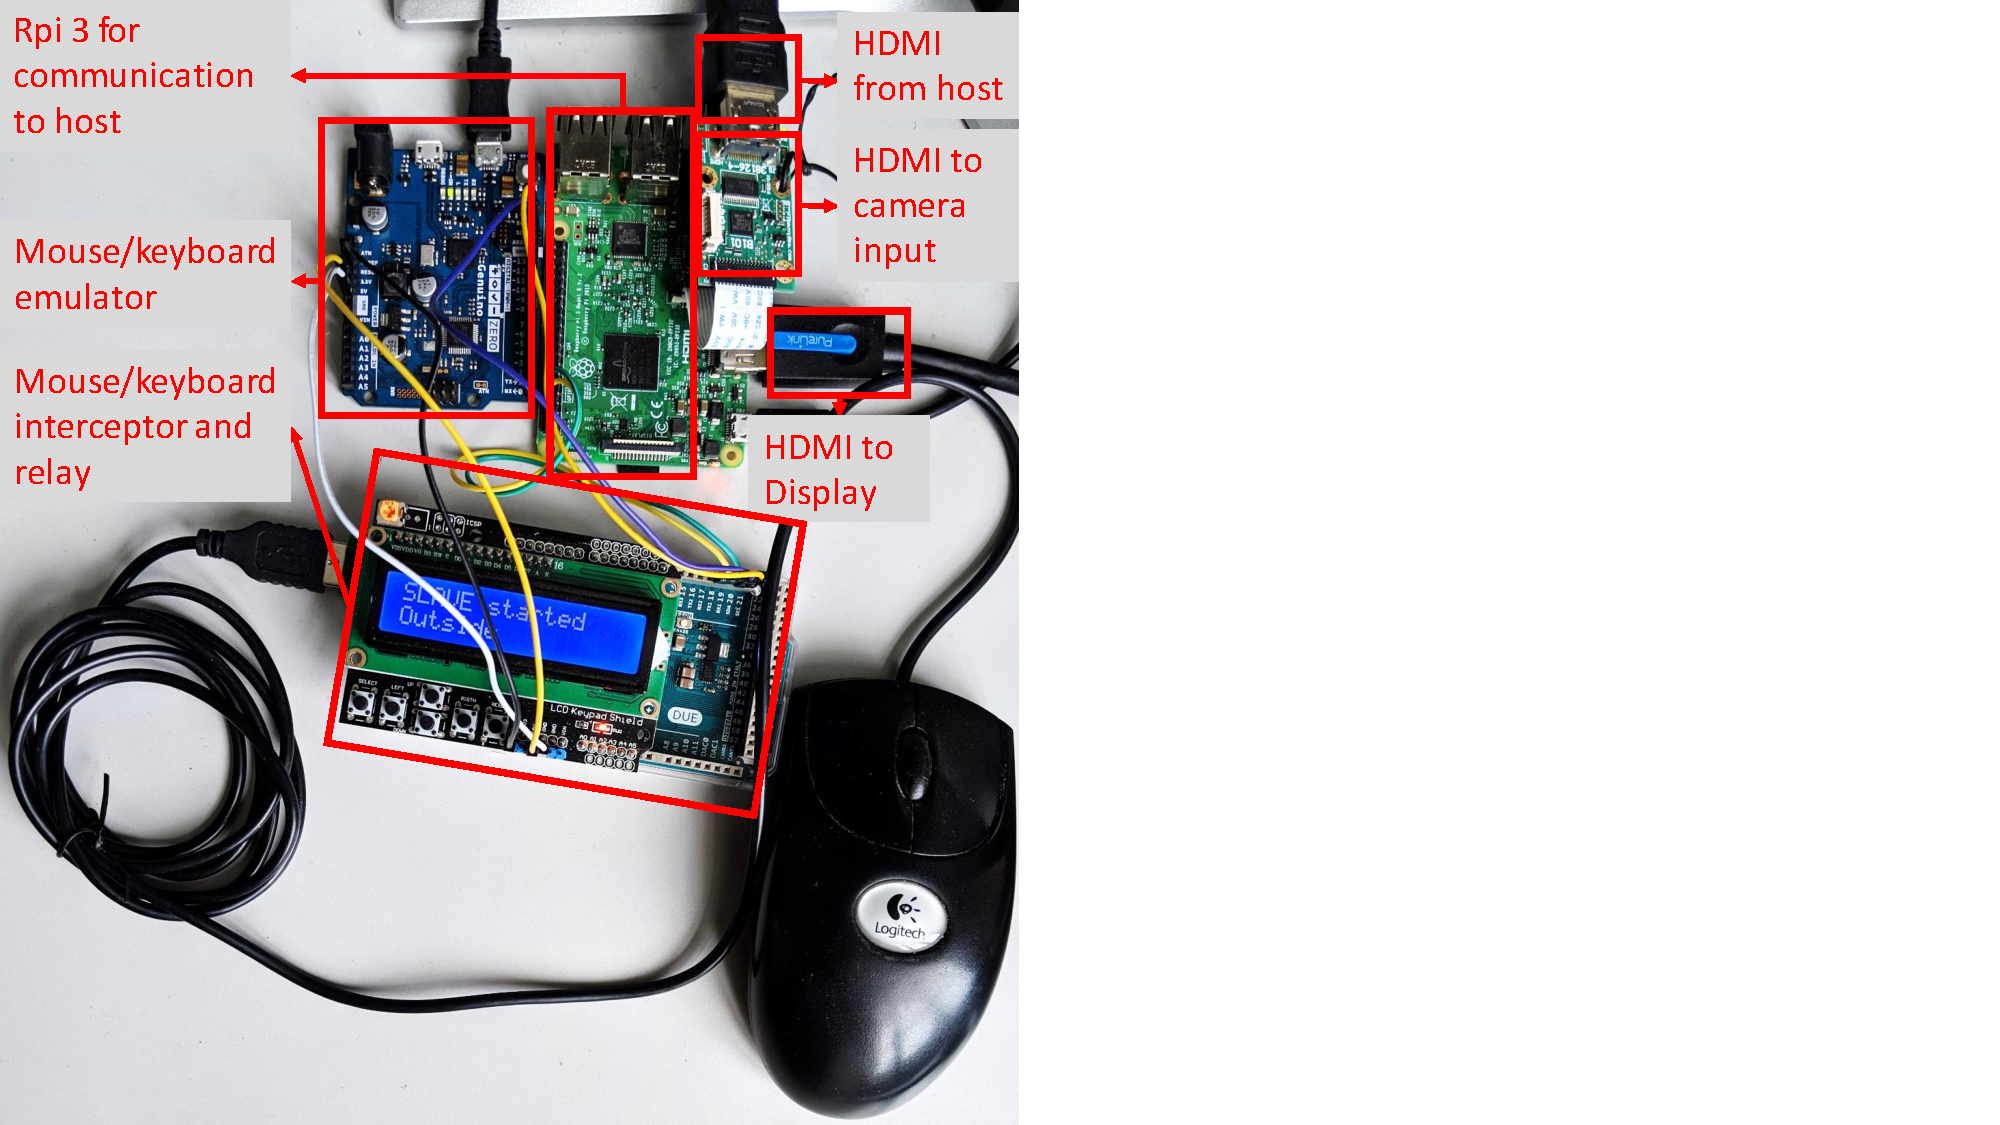
\includegraphics[trim={0 0 15cm 0}, clip, width=\linewidth]{setUp.pdf}
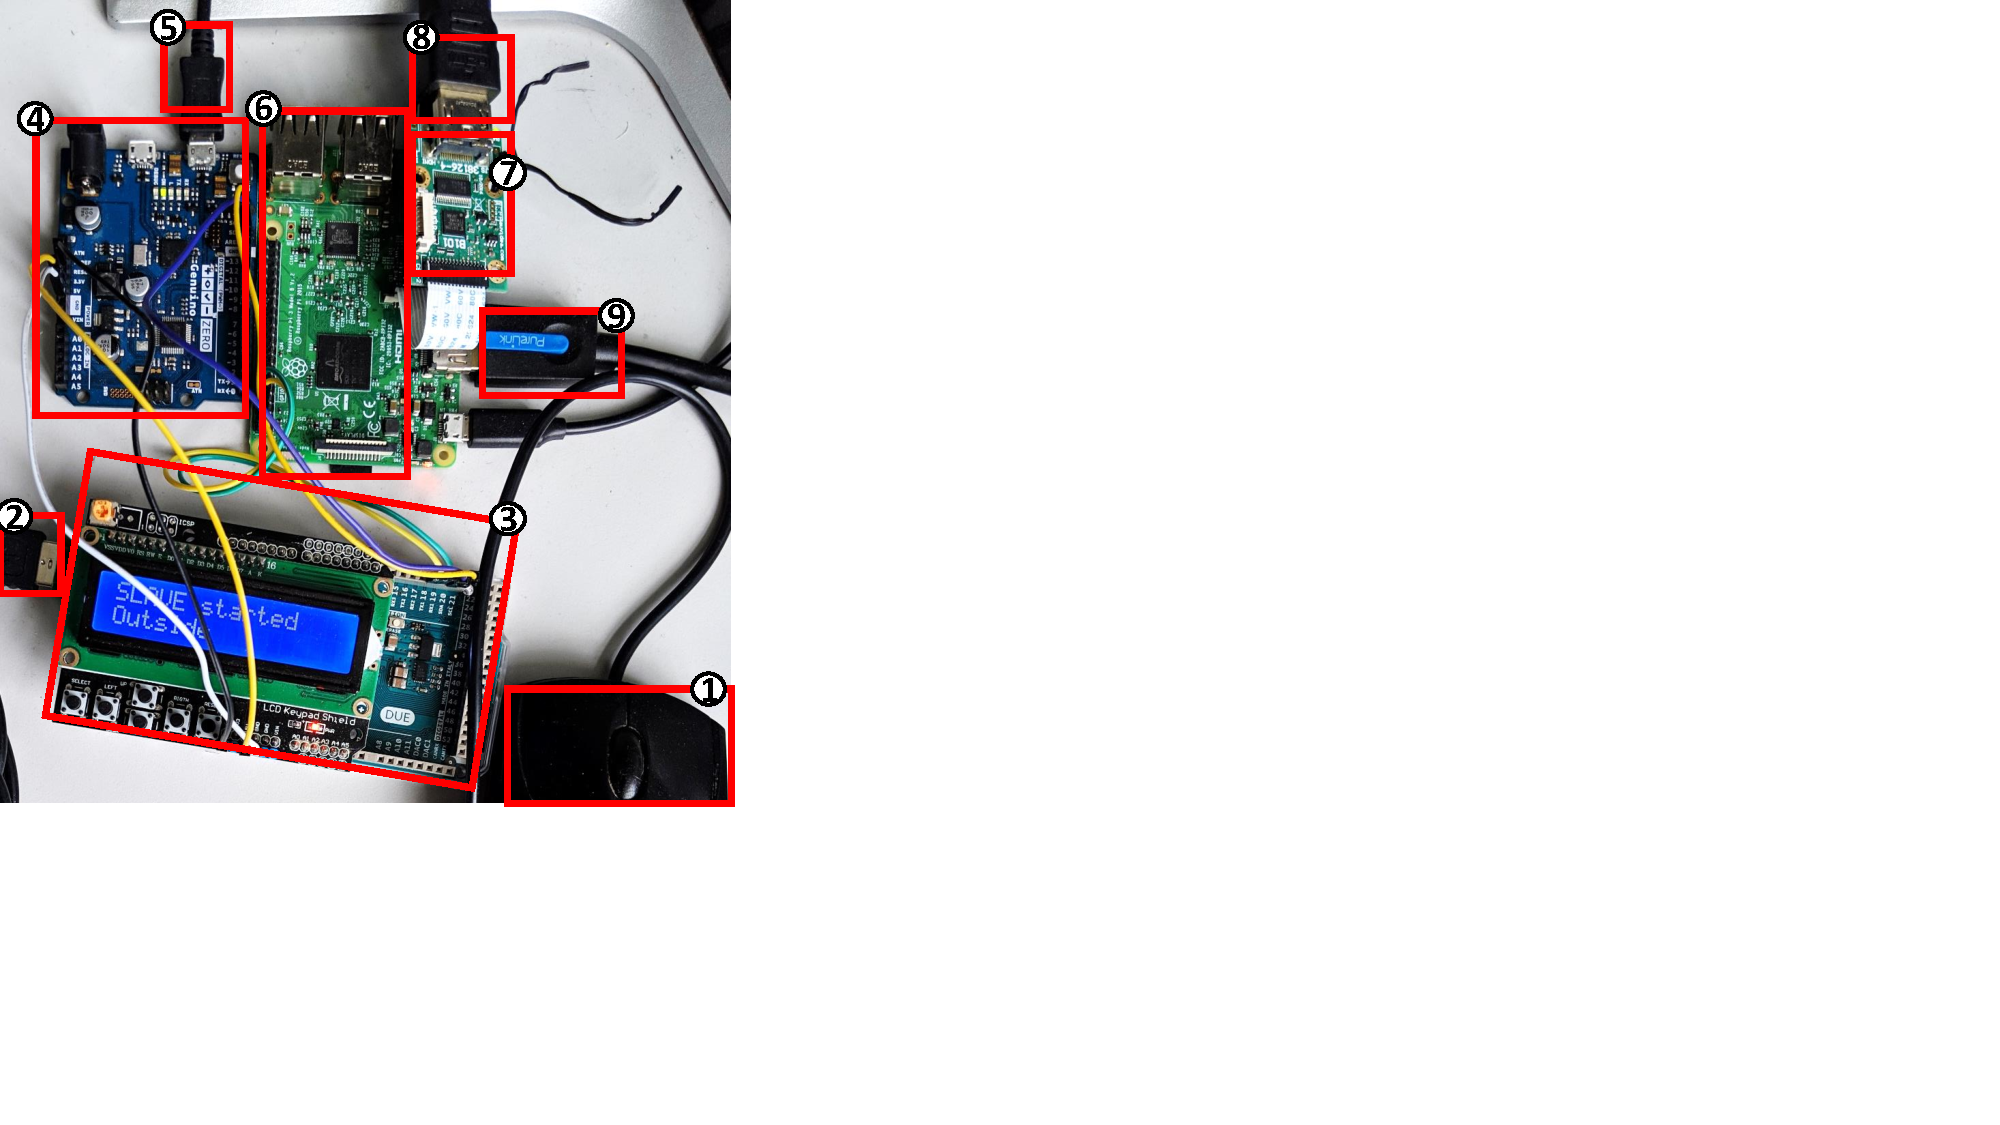
\includegraphics[trim={0 5cm 21.5cm 0}, clip, width=0.75\linewidth]{setUp_1.pdf}
\caption{\textbf{\name prototype}. The figure shows \name prototype that employs Arduino Due and Zero microcontroller board and a Raspberry Pi 3 SBC. The highlighted numbers correspond to the labels in Figure~\ref{fig:prototypeArch}.}
\label{fig:prototype}
\centering
\end{figure}
\fi


In this section, we describe our prototype implementation of \name as an auxiliary device. Figure~\ref{fig:prototype} depicts the \name prototype. The prototype \device is connoted to a desktop computer with 3.40 GHz Intel Core i7-6700 processor with 8 GB RAM running Ubuntu 18.04.2 LTS. The \device uses off-the-shelf components that has the following components and interfaces:

\begin{mylist}

  \item \textbf{Input interceptor.} The input interceptor is composed of a Arduino Due (\three) and an Arduino Zero (\four) that is connected to the input device over \usb (\two) interface. The input interceptor has a \usb out interface that connects to the host (\five) that relays all the user inputs to the host. 

  \item \textbf{HDMI interceptor.} The HDMI interceptor (\seven) is implemented using a B101 HDMI to CSI-2 Bridge~\cite{b101} that takes the HDMI channel (\eight) from the host and convert it to camera input signal to the Raspberry Pi 3.  
  
      \item \textbf{Compute component.} We use a Raspberry Pi 3 to implement the compute device that executes all the \device logic that includes analyzing the HDMI frame, composing the overlays, executing \tls protocol etc. Once could use an ASIC to further improve performance and reduce the code base of the compute component. The compute device is connected to the display over HDMI (\nine) interface. The compute component is implemented using Python and Java.
\end{mylist}

Additionally, for testing we also create a simulator of the prototype that runs in pure java to emulate more UIs as a proof of concept. The emulator creates desktop mirroring emulating the HDMI intercept.